The ProtoDUNE-SP (NP04) experiment will be housed in the EHN1 building at CERN. The detector is situated at the end of the H4 beamline in the newly constructed extension of EHN1. The H4 beamline is also extended and configured to deliver either a hadron or a pure electron beam to the experiment. To produce particles in the momentum range of interest, the secondary beam from the T2 primary target is sent onto a secondary target to generate a tertiary beam. Particles in this tertiary beam are momentum- and charge-selected and transported down the H4 beamline extension to the ProtoDUNE-SP detector. 
 In this Chapter, we discuss the beam requirements, H4 tertiary beamline design and instrumentations, DAQ/trigger, and the physics run plans.  
%The beamline layout is described and illustrated in Section~\ref{sec:h4beamline}. % minimize interference between the two ProtoDUNE experiments.

%%%%%%%%%%%%%%%%%%%%%%%%%%%%%%%%%%%%%%%%%%%%%%
\section{Beam requirements}
\label{sec:beamrequirements}

%The requested beam parameters are driven by the requirement that the results from the CERN test beam should be directly applicable to the future large underground single-phase LAr detector with minimal extrapolation. The CERN test beam data will be used to evaluate the detector performance, to understand the various physics systematic effects, and to provide data for event reconstruction studies that are representative of neutrino interactions. To satisfy the requirement, the beam parameters must span a broad range of particle momenta to match the charged particle spectrum and topologies that are expected in the DUNE far detector. The particle beam composition should consist of electrons, muons, and hadrons and needs to be charge-selected. The expected momentum distributions for secondary particles from neutrino interactions are shown in Figure~\ref{fig:particlemomenta}. There is a large spread in the momentum distribution with a clear peak near 200 MeV/c momentum per particle. The desirable momentum range for ProtoDUNE-SP  is in the low momentum region. Based on the feedback and constraints from the CERN beam group, the requested beamline design allows the transport of beam particles from about 0.5 GeV/c up to 7 GeV/c. 

The CERN test beam results from ProtoDUNE-SP will be used to evaluate the detector performance,  understand the various physics systematic effects, and provide data for event reconstruction studies that are representative of neutrino interactions. 
The parameters defining the test beam are primarily driven by the requirement that these test beam results be directly applicable to DUNE's future large underground single-phase detector module(s) with minimal extrapolation.
To match the charged-particle spectrum and topologies that are expected in the DUNE far detector, the H4 tertiary beam must span a broad range of particle momenta, be composed of electrons, muons, and hadrons, and charge-selectable. 
The expected momentum distributions for secondary particles from neutrino interactions in the far detector has a large spread that ranges from a few hundred MeV/c to a few GeV/c.
The desirable range for ProtoDUNE-SP is in the low-momentum region. Based on the feedback and constraints from the CERN accelerator group, the design of the beamline extension has been developed to allow the transport of beam particles from about 0.5~GeV/c up to 7~GeV/c. 

The maximum electron drift time in the ProtoDUNE-SP TPC is about 2.25~ms. In order
to keep the  pile-up in the TPC at the percent level, the planned
beam particle rate should be below 100 Hz.  
The ProtoDUNE-SP TPC has two drift volumes separated by a cathode plane. It is desirable to aim the particle beam such
that a large fraction of the lower-energy hadronic showers are %mostly
contained in one drift volume, thus minimizing the uncertainties from
particles lost in the inactive detector materials. 
As shown in Figure~\ref{fig:beamwindow_loc}, multiple beam injection points have been explored. Based on inputs from the physics group, the larger angle (beam \# 3) w.r.t. the APA plane (Saleve side), which corresponds to about 13$^\circ$, is preferred.
Due to engineering and safety considerations, only beam \#3 will
be fully instrumented with the beam window system as described in
Sections~\ref{subsec:fc-beamplug} and ~\ref{subsec:beamwindow}.
%The angles of the beam, with respect to the APA plane
%are 3$^\circ$ (beam \#1), 8$^\circ$ (beam \#2), and 12$^\circ$ (beam \#3). 
%The remaining two beam positions will have partial installation of the beam window system. 
The remaining two beam positions do not have the beam window system installed. 
With this configuration, beam \#3 is the primary beam %where 
with which most of the physics
data will be taken.
\begin{cdrfigure}[Beam window locations]{beamwindow_loc}{Three possible beam injection points. The cryostat support structures near the beam injection points are removed in the Figure to show the interior. Beam window and beam plug are installed only for beam \# 3.}
  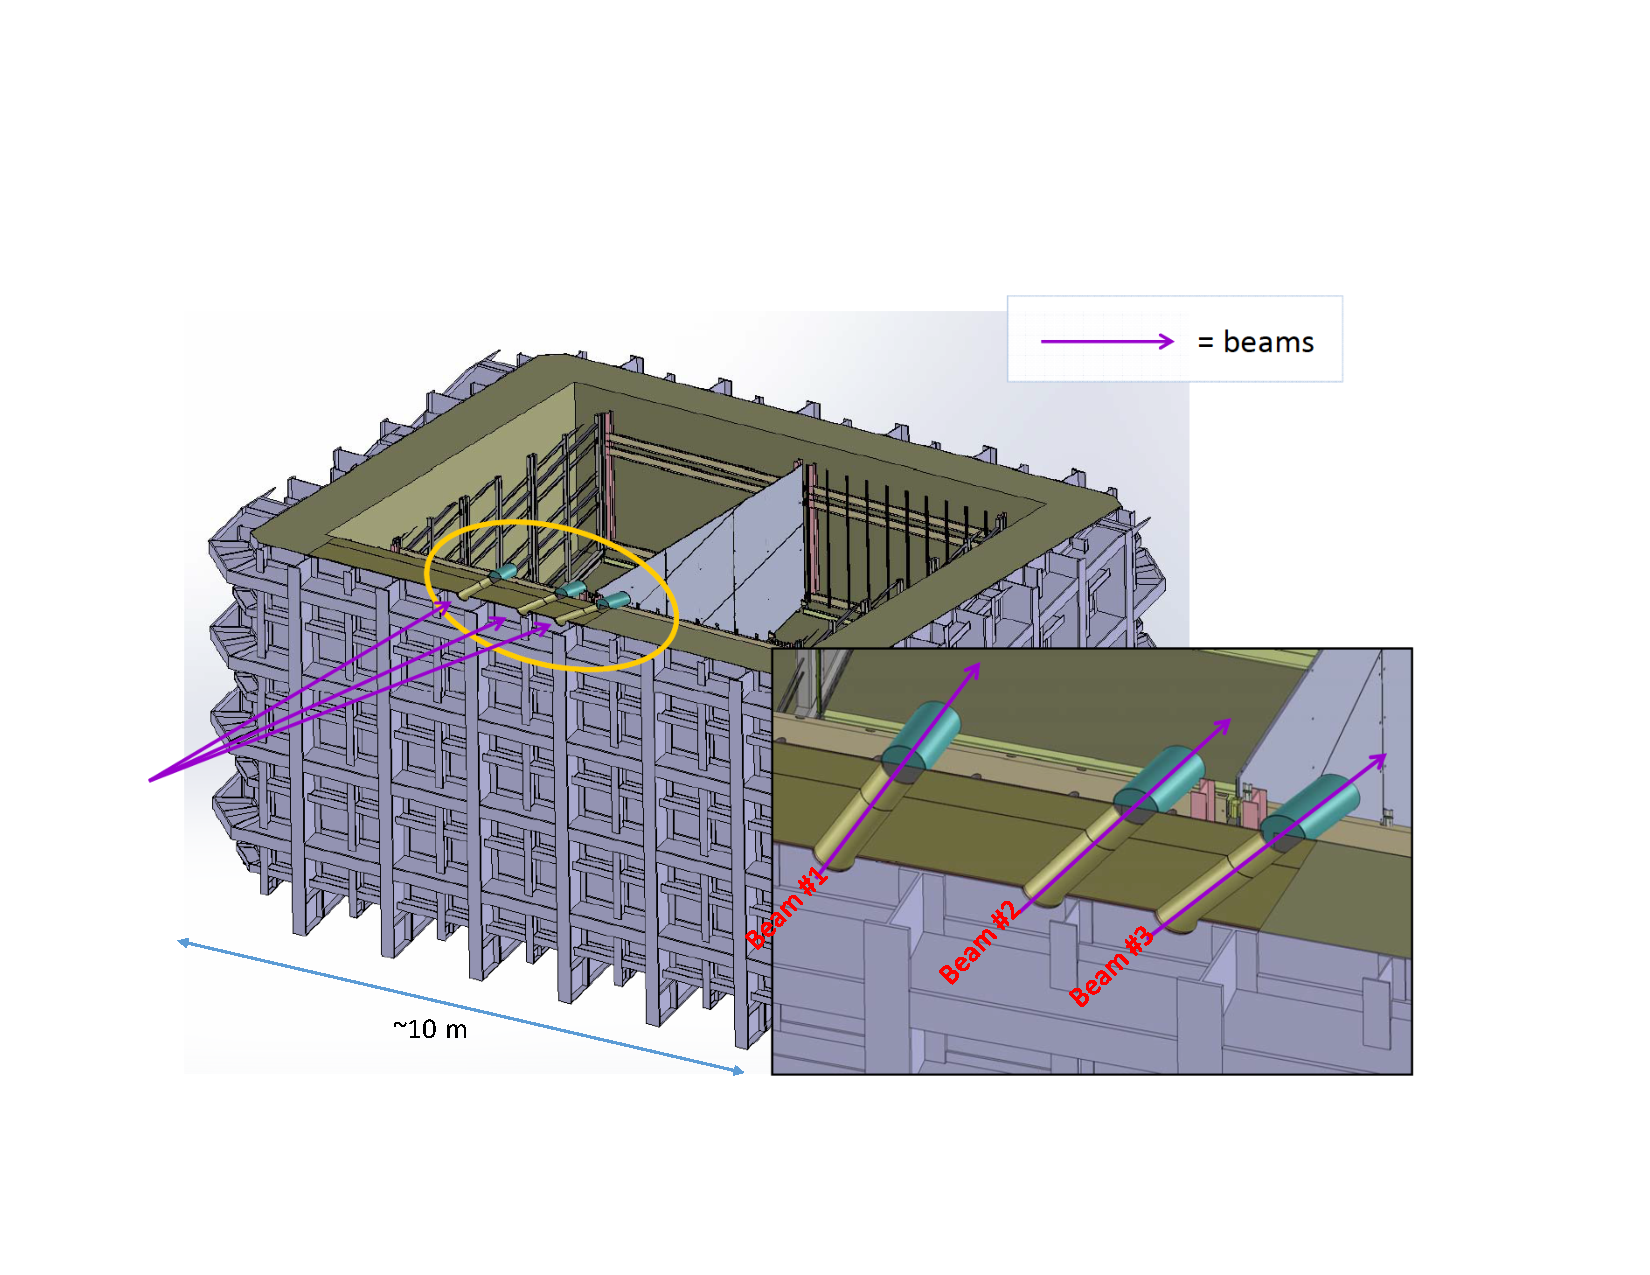
\includegraphics[width=0.9\textwidth]{beamwindow_locations.pdf}
\end{cdrfigure}
%\fixme{ Although explained in the text, this figure with three equal beam penetrations/plugs is misleading, should be modified}
A summary of the beam requirements is shown in Table~\ref{tab:beamspecs}.
\begin{cdrtable}[Particle beam requirement]{ll}{beamspecs}{Particle beam requirements. (Kaon rate is low for beam momentum below 2 GeV/c.)}
%\textbf{Parameter } & \textbf{Requirements}  \\ \hline
 Parameter & Requirements \\ \toprowrule
  Particle Types        & $e^\pm,\mu^\pm,\pi^\pm$,$(K)$,$p$  \\ \colhline
  Momentum Range   & 0.5 - 7 GeV/$c$ \\ \colhline
  Momentum Resolution   & $\Delta p/p   \le 3$ \% \\ \colhline
  Transverse Beam Size   & RMS(x,y) $\approx$ 1 cm  \\
  & (At the entrance face of the LAr cryostat) \\ \colhline
%  Beam Divergence & tbd   \\ \colhline
  Beam Entrance Position & Beam \# 3 (Figure~\ref{fig:beamwindow_loc}) - Saleve side TPC   \\ \colhline
  Rates & $\sim25 - \sim100$\,Hz     \\ \colhline
\end{cdrtable}
